\graphicspath{ {./figuresAnalysis} }
\section{Analyse fonctionnel}
\subsection{Besoin}
Prévenir le dévlopement de maladie

Il existe des modèle empyrique qui se base sur le temps d'humidité sur la feuille. difficile a déterminer par les donné méto clasique (humidité température vents etc). Le recours à un capteur d'humectation est utile dans ce cas la.

\begin{figure}[!ht]
 \centering
 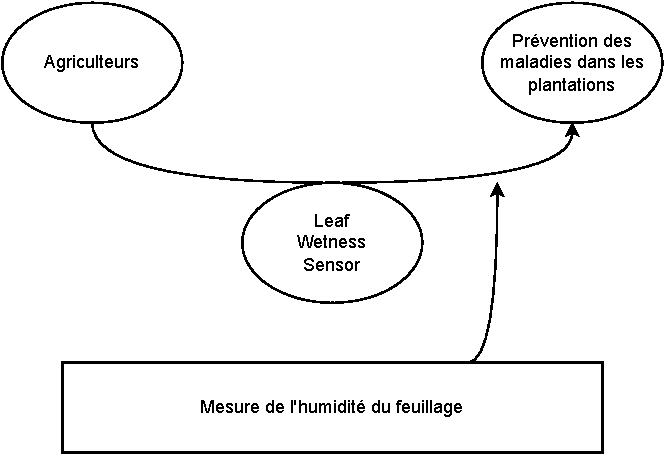
\includegraphics{DiagrammeCorne.drawio.pdf}
\end{figure}

\subsection{Diagramme pieuvre et cahier des charges}

\begin{figure}[!ht]
 \centering
 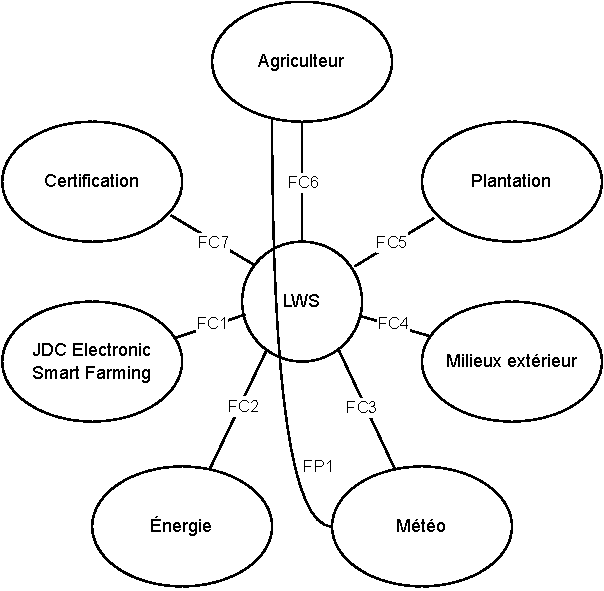
\includegraphics{DiagrammePieuvre.drawio.pdf}
\end{figure}

\begin{table}[!h]
\begin{center}
\resizebox{\columnwidth}{!}{%
\begin{tabular}{|l|l|p{5cm}|l|}
\hline
 & \textbf{Fonctions} & \textbf{Critères} & \textbf{Niveaux}\\
\hline
\textbf{FP1} &Mesurer l'humectation des feuilles & Mesure d'humidité relative d'une surface & RH de 0\% à 100\%  résolution de 0.5\%  précision +- 0.25\%\\
\hline
\multirow{5}{*}{\textbf{FC1}} & S'intégrer dans l'environement Smart Farming JDC & Interface  de sortie I2C & Baud rate 100KHz. Adresse configurable\\\cline{3-4}
 &  & Structure de registre normalisé, & (voir doc JDC)\\\cline{3-4}
 &  & Démarrage de la mesure et acquisition après un temps. & 50ms pour la capture de la mesure\\\cline{3-4}
 &  & Connecteur JDC & Sortie 4 fil avec  VCC,GND,SDA,SCL\\\cline{3-4}
 &  & Alimentation normalisé & Tesion 3.3V\\\cline{3-4}
\hline
\textbf{FC2} & Consommer peu d'énergie & Courant maximum établit en fonctionnement & 1 mA\\
\hline
\textbf{FC3} & Eviter les faux positifs du à la métérologie & L'humidité de l'aire ne doit pas influencer la mesure & L'incidence de RH de l'aire < précision (0.25\%)\\
\hline
\textbf{FC4} & Résister aux milieux extérieur & Le capteur est protégé des intempéries et supporte une utilisation extérieur & Etanche IP44\\
\hline
\textbf{FC5} & S'intègrer dans les plantations & La taille du capteur ne doit pas gêner l'exploitation des plantations & Envergure maximum de 20cm\\
\hline
\textbf{FC6} & Etre facile d'installation & Le capteur doit pouvoir être installer par des agriculteurs sans formation technique & Système d'atache et un seul connecteur a brancher\\
\hline
\textbf{FC7} & Etre Certifié & Le capteur doit être certifié pour être proposé sur le marché & Certification EM,CE\\
\hline
\end{tabular}
}
\end{center}
\end{table}

\subsection{Diagramme Fast}

\begin{figure}[!ht]
 \centering
 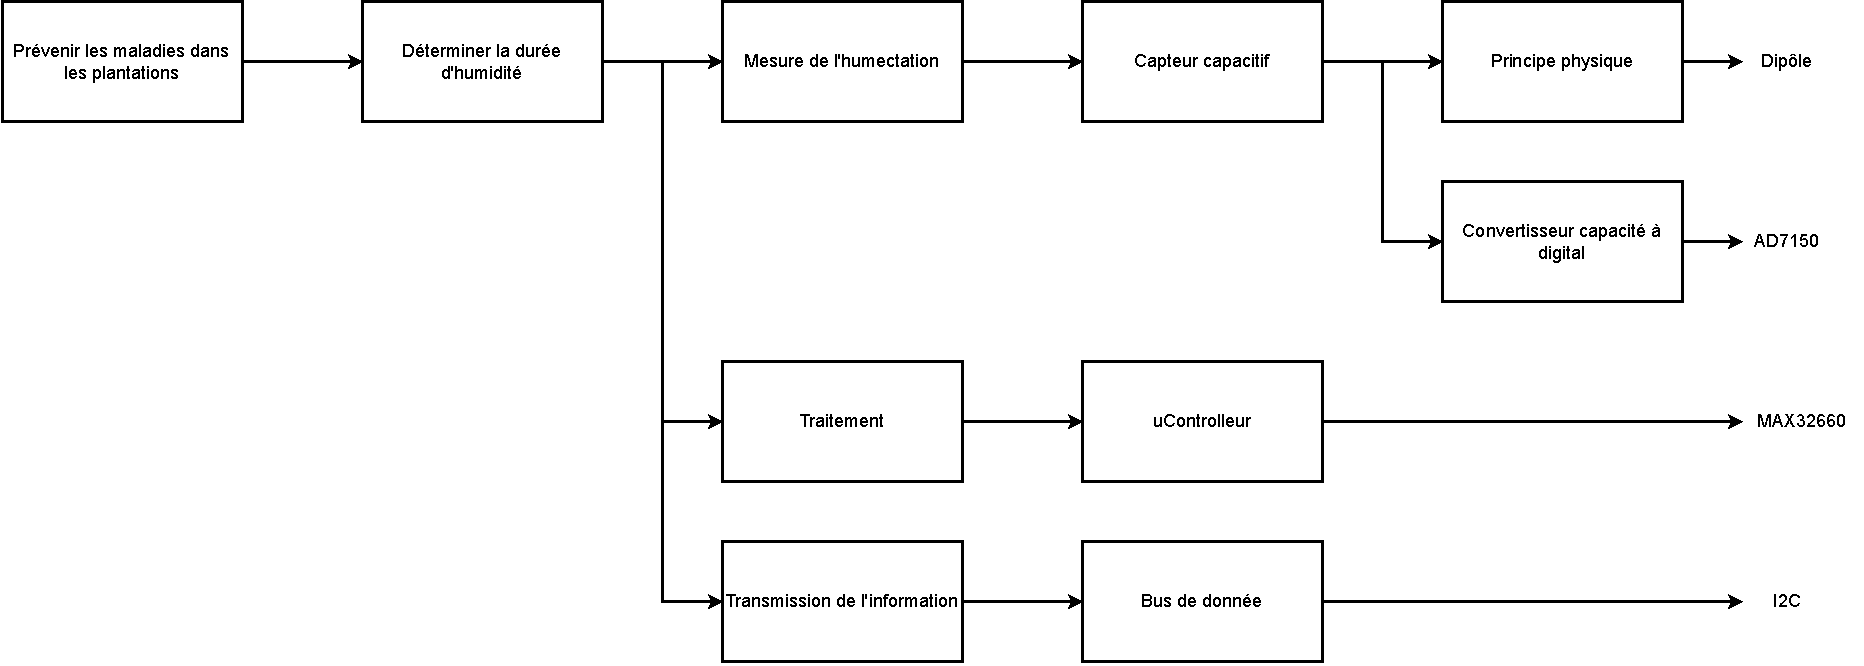
\includegraphics[width=16cm]{DiagrammeFAST.drawio.pdf}
\end{figure}

\subsection{Schéma fonctionnel}

\begin{figure}[!ht]
 \centering
 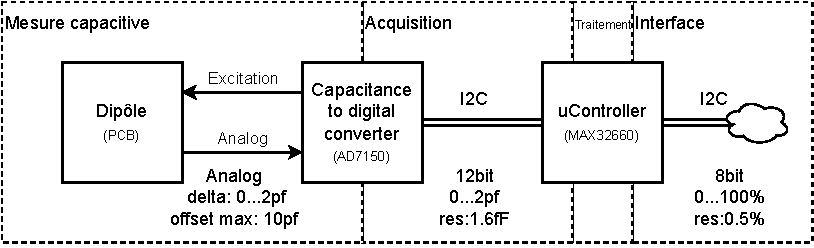
\includegraphics[width=16cm]{SchemaBlock.drawio.pdf}
\end{figure}
